\documentclass{beamer}
\usepackage[utf8]{inputenc}

\usepackage{utopia} %font utopia imported

\usetheme{Madrid}
\usecolortheme{default}

%------------------------------------------------------------
%This block of code defines the information to appear in the
%Title page
\title[MA-473 Term Paper] %optional
{Computation of American Type of Floating Strike Asian Option}

\subtitle{Numerical Methods}
\author[Rupam Sahu, Ayush Dalia, Aditya Raj] % (optional)
{Rupam Sahu\inst{1} \and Ayush Dalia\inst{2} \and Aditya Raj\inst{3}}



\date[14 April 2021] % (optional)
{MA473 Term Paper Presentation, April 2021}

%\logo{\includegraphics[height=1.5cm]{lion-logo.jpg}}

%End of title page configuration block
%------------------------------------------------------------



%------------------------------------------------------------
%The next block of commands puts the table of contents at the 
%beginning of each section and highlights the current section:

\AtBeginSection[]
{
  \begin{frame}
    \frametitle{Table of Contents}
    \tableofcontents[currentsection]
  \end{frame}
}
%------------------------------------------------------------


\begin{document}

%The next statement creates the title page.
\frame{\titlepage}
%-----------------------------------------------------------
%the title page
\begin{frame}
\frametitle{Introduction}
    \begin{itemize}
        \item Problem of pricing American Style Asian Option
        \item Asian Options are grouped in path-dependent options.
        \item Pricing PDEs for arithmetic average cannot be solved analytically
    \end{itemize}
\end{frame}
%----------------------------------------------------------
%---------------------------------------------------------
%-----------------------------------------------------------
\begin{frame}
\frametitle{Free Boundary Problem}
    \begin{itemize}
        \item Solution of parabolic equation with free boundary $S_{f}(t,A)$
        \item \begin{equation}\frac{\partial V}{\partial t} + \frac{\sigma^{2}}{2}S^{2}\frac{\partial^{2} V}{\partial S^{2}} + (r-q)S\frac{\partial V}{\partial S} + \frac{S-A}{t}\frac{\partial V}{\partial A} - rV = 0
        \end{equation}
        \item 
           \begin{equation}
               V(t,0,A) = 0,  
           \end{equation} for any $A>0 and 0<t<T$
         \item
            \begin{equation}
                \frac{\partial V}{\partial S}(t, S_{f}(t,A),A) = 1, V(t,S_{f}(t,A),A) = S_{f}(t,A) - A
            \end{equation}
        \item
            \begin{equation}
                V(T,S,A) = max(S-A,0), S,A > 0.
            \end{equation}
        \item $A_{t} = \frac{1}{t}\int_{0}^{t}S_{u}du$ 
    \end{itemize}
\end{frame}
%----------------------------------------------------------
\begin{frame}\frametitle{Free Boundary Problem}
    \begin{itemize}
        \item Perform dimension reduction by introducing a new time variable $\tau$ and a similarity variable x
        \item $\tau =  T-t$ , $x = \frac{A}{S}$, $W(x,\tau) = \frac{V(t,S,A)}{A}$
        \item $\frac{1}{\rho(t)} < x < \infty$ , $\tau\epsilon(0,T)$, $\rho(\tau) = \frac{S_{f}(T - \tau, A)}{A}$
        \item Introduce a new state variable $\xi$ and an auxiliary function $\Pi(\xi,\tau) = W(x,\tau) + x\frac{\partial W}{\partial x}(x,\tau)$
        \item Here, $\xi = ln(\rho(\tau)x)$
    \end{itemize}
\end{frame}
%---------------------------------------------------------
\begin{frame}\frametitle{Transformation to IBVP}
    \begin{itemize}
        \item \begin{equation}
            \frac{\partial \Pi}{\partial \tau} + \alpha(\xi, \tau)\frac{\partial \Pi}{\partial \xi} - \frac{\sigma^{2}}{2}\frac{\partial^{2} \Pi}{\partial \xi^{2}} + \beta(\xi, \tau)\Pi = 0, \xi > 0, \tau\epsilon(0,T)
            \end{equation}
        \item \begin{equation} 
            \Pi(0,\tau) = -1, \Pi(\infty,\tau) = 0, \Pi(\xi, 0) = -1 for \xi < ln(\rho(0))
        \end{equation}
        \item $\alpha$ and $\beta$ coefficients are defined as follows - 
            
                \begin{equation}
                    \alpha(\xi,\tau) = \frac{\u{\rho(\tau)}}{\rho(\tau)} + r-q - \frac{\sigma^{2}}{2} - \frac{\rho(\tau)e^{-\xi} - 1}{T - \tau}, \beta(\xi, \tau) = r + \frac{1}{T - \tau}
                \end{equation}
        \item $\rho(\tau)$ and $\Pi$ should fulfill the constraint - 
        \begin{equation}
            \rho(\tau) = \frac{1 + r(T-\tau) + \frac{\sigma^{2}}{2}(T-\tau)\frac{\partial \Pi}{\partial \xi}(0,\tau)}{1 + q(T- \tau)} , \rho(0) = max(\frac{1 + rT}{1 + qT},1)
        \end{equation}
    \end{itemize}
    
\end{frame}
%--------------------------------------------------------------
\begin{frame}{Transformation to IBVP}
    \begin{itemize}
        \item solution $\Pi$ to the problem (5)-(8) is continuous for $t > 0$
        \item Discontinuity occurs at $P^{*} = (ln(\rho(0)), 0)$
        \item Derivatives of the solution exist and are sufficiently smooth in [0,L]×[0, T)
        \item For times t → 0^{+} (i.e. $when \tau$ → T ) the coefficients $\alpha, \beta$ become unbounded
    \end{itemize}
\end{frame}
%---------------------------------------------------------------
\begin{frame}{Finite Difference Schemes}
\begin{equation}
    \frac{y_{i}^{j+1} - y_{i}^{j}}{k} + \alpha_{i}^{j+1}\frac{y_{i+1}^{j+1} - y_{i-1}^{j+1}}{2h} - \frac{\sigma^{2}}{2}\frac{y_{i+1}^{j+1} - 2y_{i}^{j+1} + y_{i-1}^{j+1}}{h^{2}} + \beta^{j+1}y_{i}^{j+1} = 0
\end{equation}
\begin{equation}
    y_{0}^{j+1} = -1, y_{N}^{j+1} = 0; y_{i}^{0} = \begin{cases}
    -1 &\text{,for $\xi \leq ln(\rho(0))$}\\
    0 &\text{,otherwise}
    \end{cases}
\end{equation}
\begin{equation}
    \alpha_{i}^{j+1} = \frac{z^{j+1} - z^{j}}{kz^{j+1}} + r - q - \frac{\sigma^{2}}{2} - \frac{z^{j+1}exp(-\xi) - 1}{T - \tau_{j+1}}, \beta^{j+1} = r + \frac{1}{T - \tau_{j+1}}
\end{equation}
\begin{equation}
    z^{j+1} - \frac{1 + r(T-\tau_{j+1})}{1 + q(T-\tau_{j+1})} - \frac{\sigma^{2}}{2}\frac{T - \tau_{j+1}}{1 + q(T-\tau_{j+1})}\frac{-3y_{0}^{j+1} + 4y_{i}{j+1} - y_{2}^{j+1}}{2h} = 0
\end{equation}
\end{frame}
%This block of code is for the table of contents after
%the title page to get correct value.



%---------------------------------------------------------


%---------------------------------------------------------
%Example of the \pause command
\begin{frame}
\frametitle{Algorithms}
\tableofcontents
\end{frame}
%---------------------------------------------------------


\section{Predictor-Corrector Scheme}

%---------------------------------------------------------
%Changing visivility of the text
\begin{frame}
\frametitle{Predictor-Corrector}
In Predictor corrector scheme we first predict the value using some explicit method then use the predicted value to get correct value.

\begin{itemize}
    \item<1-> Predictor\\
   We introduce a spatial node $\xi_{-1}$ and let the solution be known at time level $\tau_{j}$.Rewriting equation 8 as:
    \[(1+q(T-\tau_{j+1}))z^{j+1}=1+r(T-\tau_{j+1})+\frac{\sigma^2}{2}(T-\tau_{j+1})\frac{y_{1}^{j+1}-y_{-1}^{j+1}}{2h}    \hspace{4mm}(13)\] 
   
     To use the fact that $\Pi(0,\tau)=-1$(constant) so $\frac{\partial \Pi}{\partial \tau}=0$ at i=0 
      \[\alpha_{0}^{j+1}\frac{y_{1}^{j+1}-y_{-1}^{j+1}}{2h}-1+\frac{\sigma^2}{2}\frac{y_{1}^{j+1}-2y_{0}^{j+1}+y_{-1}^{j+1}}{h^2}+\beta^{j+1}y_{0}^{j+1}=0    \hspace{4mm}(14)\] 
      Using 13 and 14
      \[y_{1}^{j+1}=(\frac{2\alpha_{0}^{j+1}h^2}{\sigma^4}+\frac{2h}{\sigma^2})(qz^{j+1}-r+\frac{z^{j+1}-1}{T-\tau_{j+1}})-\frac{\beta^{j+1}h^2}{\sigma^2}-1   \hspace{4mm}(15)\]
   
\end{itemize}
\end{frame}

%---------------------------------------------------------


%---------------------------------------------------------
%Example of the \pause command
\begin{frame}
 Instead of implicit we will use explicit variant for i=1 
      \[\frac{y_{1}^{j+1}-y_{1}^{j}}{k}+\alpha_{1}^{j+1}\frac{y_{2}^{j}-y_{0}^{j}}{2h}-\frac{\sigma^2}{2}\frac{y_{2}^{j}-2y_{1}^{j}+y_{0}^{j}}{h^2}+\beta^{j+1}y_{1}^{j}=0.    \hspace{4mm}(16)\]
        As $\alpha_{i}^{j+1}$ can be written in terms of $z^{j+1}$ equation 15 and 16 are non linear systems for unknowns $y_{1}^{j+1}$ and $z^{j+1}$.This can be used as predicted value of $y_{1}^{j+1}\leftrightarrow \overline{y}_{1}^{j+1}$ and $z^{j+1}\leftrightarrow \overline{z}^{j+1}$.
        \begin{itemize}
    \item<1-> Corrector\\
   Now using implicit scheme:
   \[\frac{y_{i}^{j+1}-y_{i}^{j}}{k}+\overline{\alpha}_{i}^{j+1}\frac{y_{i+1}^{j+1}-y_{i-1}^{j+1}}{2h}-\frac{\sigma^2}{2}\frac{y_{i+1}^{j+1}-2y_{i}^{j+1}+y_{i-1}^{j+1}}{h^2}+\beta^{j+1}y_{i}^{j+1}=0.    (17)\]
   where 
   \[\overline{\alpha}_{i}^{j+1}=\frac{\overline{z}^{j+1}-z^{j}}{k\overline{z}^{j+1}}+r-q-\frac{\sigma^2}{2}-\frac{\overline{z}^{j+1}exp(-\xi_{i})-1}{T-\tau_{j+1}} \hspace{4mm}(18)\]
   The corrected solution $y_{i}^{j+1}$ and $z^{j+1}$ is used to obtain solution in next time layer.
\end{itemize}
        
\end{frame}
%---------------------------------------------------------

\section{Newton-Rhapson method}

%---------------------------------------------------------
%Highlighting text
\begin{frame}
\frametitle{Newton-Rhapson}
    \begin{itemize}
    \item<1-> Step1\\
Eliminating the known boundary values $y_{0}^{j+1}=-1$ and $y_{N}^{j+1}=0$ from 9.From 12 we obtain a nonlinear system of N unknowns $y_{i}^{j+1}, i=1,2,..N-1$ and $z^{j+1}$ denoted by $Y^{l}$ at the l-th iteration.
\item<1-> Step2\\
solve the equation $F^{l}=0$ with $F^{l}=(F_{1}^{l} F_{2}^{l})^{T}$ where $F_{1}^{l}$ corresponds to equation 9 and $F_{2}^{l}$ corresponds to equation 12.\\
Applying Newton method in the following form $J^{l}(Y^{l+1}-Y^{l})=-F^{l}$ with $J=\begin{pmatrix}
J_{11}^l & J_{12}^l\\
J_{21}^{l} & J_{22}^l
\end{pmatrix}$ where\\
\\



\end{itemize}



\end{frame}
\begin{frame}

\begin{figure}[!htb]
	\centering 
	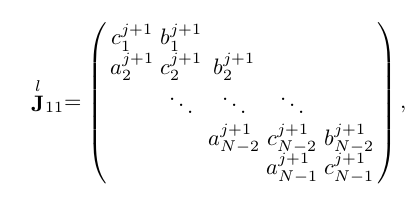
\includegraphics[width=0.7\linewidth]{j11.png}
	
\end{figure}
\end{frame}
%--------------------------------------------------------%
\begin{frame}

\begin{figure}[!htb]
	\centering 
	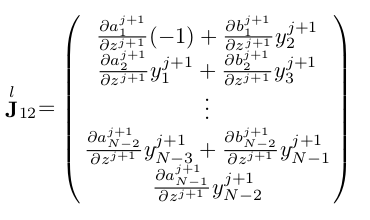
\includegraphics[width=0.7\linewidth]{image1.png}
	\[
        J_{21}^{l} = (-\frac{\sigma^{2}}{Dh},\frac{\sigma^{2}}{4Dh},0,0..0) ,D=q+\frac{1}{T-\tau^{j+1}}\\
        J_{22}^l=1
    \]
\end{figure}
\end{frame}
%--------------------------------------------------------
\begin{frame}
    \begin{equation}
        a_{i}^{j+1} = -\frac{1}{2h}(\frac{z^{j+1} - z^{j}}{kz^{j+1}} + r - q - \frac{\sigma^{2}}{2}) -\frac{\sigma^2}{2h^{2}} + d_{i}^{j+1}
    \end{equation}
    \begin{equation}
        c_{i}^{j+1} = \frac{1}{k} + \frac{\sigma^2}{h^{2}} + r + \frac{1}{T - \tau_{j+1}}
    \end{equation}
    \[
        b_{i}^{j+1} = \frac{1}{2h}(\frac{z^{j+1} - z^{j}}{kz^{j+1}} + r - q - \frac{\sigma^{2}}{2}) - \frac{\sigma^2}{2h^{2}} + d_{i}^{j+1}\\
        \hspace{25mm}d_{i}^{j+1}=\frac{1}{2h}\frac{(z^{j+1}exp(-\xi_{i})-1)}{T-\tau_{j+1}}
    \]
    \\Repeat the process until $\abs{Y^{l+1}-Y^{l}}<tol$ is satisfied.
\end{frame}
%----------------------------------------------------%
\begin{frame}
\frametitle{Mesh Refinement Analysis and CR of Newton Method}
\begin{figure}[!htb]
	\centering 
	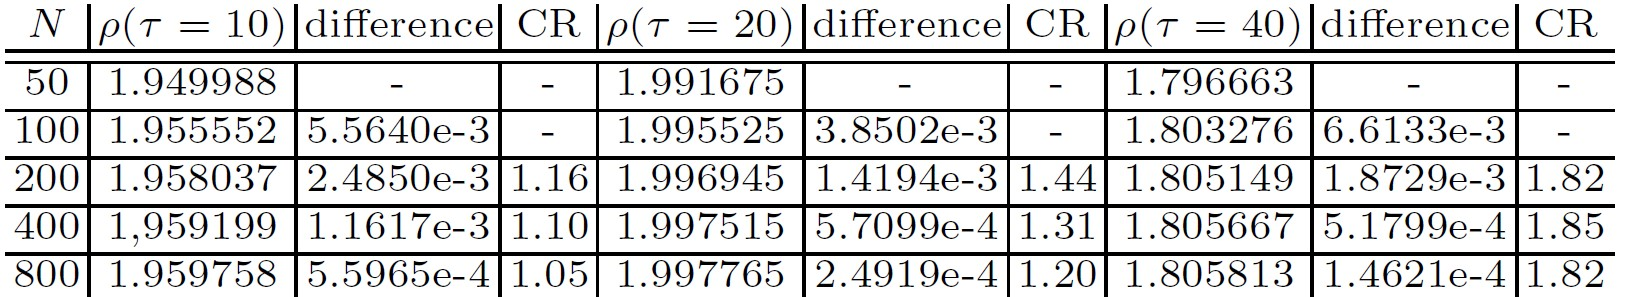
\includegraphics[width=1\linewidth]{mesh_refinement_analysis_CR.jpg}
	
\end{figure}
\end{frame}
%--------------------------------------------------
\begin{frame}{Numerical Experiments}
    
\begin{figure}[!htb]
	\centering 
	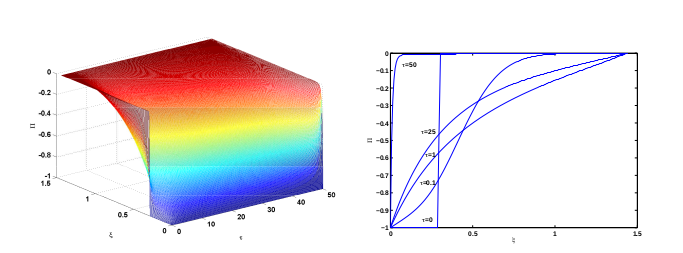
\includegraphics[width=0.7\linewidth]{image2.png}

\end{figure}
Parameter values $r=0.06,q=0.04,\sigma=0.2$ and $T=50$.
The left figure is showing value of $\Pi$ for different values of $\xi$ and $\tau$ using Newton method for $N=200,M=500$.It can be seen that $\Pi$ increases with increasing value of $\xi$.\\
The right figure is showing how $\Pi$ changes with $\xi$ for a fixed value of $\tau=0,0.1,10,25,50$.

\end{frame}
\end{document}